\documentclass{beamer}
\usepackage[utf8]{inputenc}
\usepackage{csvsimple}

\usetheme{Madrid}
\usecolortheme{default}

%------------------------------------------------------------
%This block of code defines the information to appear in the
%Title page
\title[LSTM vs Econometrics] %optional
{Carried away by long short-term memory}

\subtitle{Comprehensive comparison of LSTM against classical models}

\author[A.~Aleynikov \and S.~Mirzoev] % (optional)
{Anton~Aleynikov \and Sergey~Mirzoev}

\institute[ETH] % (optional)
{
  MSc Quantitative Finance\\
  ETH Zürich \& University of Zürich
}

\date[AQF 2023] % (optional)
{Applied Quantitative Finance, December 2023}

\logo{
\includegraphics[height=0.7cm]{figure/eth_uzh}}

%End of title page configuration block
%------------------------------------------------------------



%------------------------------------------------------------
%The next block of commands puts the table of contents at the 
%beginning of each section and highlights the current section:

\AtBeginSection[]
{
  \begin{frame}
    \frametitle{Table of Contents}
    \tableofcontents[currentsection]
  \end{frame}
}
%------------------------------------------------------------


\begin{document}

%The next statement creates the title page.
\frame{\titlepage}


%---------------------------------------------------------
%This block of code is for the table of contents after
%the title page
\begin{frame}
\frametitle{Table of Contents}
\tableofcontents
\end{frame}
%---------------------------------------------------------

\section{Introduction}

\begin{frame}{Abstract}
    \begin{itemize}
        \item Carry trade challenges FX market efficiency by exploiting interest rate differentials.
        \item Based on Wang et al. (2021), LSTM outperformed traditional models, which doesn't hold as per our research.
        \item Post-2008 crisis, excess carry trade returns deteriorated, impacting uncovered interest rate parity.
    \end{itemize}
\end{frame}

\begin{frame}{Introduction}
    \begin{itemize}
        \item Carry trade influences forex dynamics; excess returns from it pose a challenge to the market efficiency hypothesis.
        \item This research uses LSTM networks to forecast carry trade returns, a novel approach.
        \item Objective: Improve understanding of carry trade dynamics and evaluate LSTM's effectiveness.
    \end{itemize}
\end{frame}

\begin{frame}{Research Focus}
    \begin{itemize}
        \item Literature review on carry trade and forecasting models.
        \item Comparison of LSTM with linear and threshold regression models.
        \item Methodology, results, and implications for forex market efficiency and carry trade strategies.
    \end{itemize}
\end{frame}

\section{Carry trade \& Economic background}

\begin{frame}{Economic Foundations}
    \begin{itemize}
        \item Fundamental concepts: Efficient Market Hypothesis (EMH) and Uncovered Interest Parity (UIP).
        \item EMH suggests markets efficiently reflect all information, challenging consistent profit through analysis.
        \item UIP explores the relationship between interest rates and exchange rates, expecting equal returns across currencies when not hedged.
    \end{itemize}
\end{frame}

\begin{frame}{Efficient Market Hypothesis (EMH)}
    \begin{itemize}
        \item EMH categorises into Weak, Semi-Strong, and Strong forms.
        \item \textbf{Weak Form:} Past price and volume info already in stock prices.
        \item \textbf{Semi-Strong Form:} All public info reflected, challenging fundamental and technical analyses.
        \item \textbf{Strong Form:} All public or private info fully reflected, even insider information.
    \end{itemize}
\end{frame}

\begin{frame}{EMH Implications for Investors}
    \begin{itemize}
        \item Challenges effectiveness of active trading strategies.
        \item Supports the idea of a passive buy-and-hold approach.
        \item Investors may not consistently achieve higher-than-average returns.
    \end{itemize}
\end{frame}

\begin{frame}{Uncovered Interest Parity (UIP)}
    \begin{itemize}
        \item Explores the relationship between interest rates and exchange rates.
        \item Expectation: Equal returns on investments across currencies when not hedged.
    \end{itemize}

    \begin{block}{Mathematical expression}
    \( \mathbf{E}(\Delta e_{t+1}) = i_t - i^*_t \), where $i_t$ is the domestic interest rate and $i^*_t$ is the foreign interest rate, $\Delta e_{t+1}$ is the logged exchange rate difference
    \end{block}
\end{frame}

\begin{frame}{UIP Empirical Studies}
    \begin{itemize}
        \item Mixed evidence regarding the validity of UIP.
        \item Various factors influence the observed relationship between interest and exchange rates.
    \end{itemize}
\end{frame}

\begin{frame}{Summary}
    \begin{itemize}
        \item EMH challenges active trading, supporting passive approaches.
        \item UIP explores the interest rate-exchange rate relationship with mixed empirical evidence.
    \end{itemize}
\end{frame}

\begin{frame}{Carry Trade and Excess Returns}
    \begin{itemize}
        \item Carry trade, an arbitrage strategy based on interest rate differentials, is extensively studied in financial economics.
        \item Returns linked to exchange rate changes and interest rate differentials.
        \item Challenges the Efficient Market Hypothesis (EMH).
        \item Evidence suggests long-term Uncovered Interest Parity (UIP) may lead to excess carry trade return reversal \cite{wang2021machine}.
    \end{itemize}
\end{frame}

\section{Methodology}

\begin{frame}{Methodology Overview}
    \begin{block}{Dataset}
        \begin{itemize}
            \item Spans 1990–2019, covers 11 G10 countries.
            \item Exchange rate, one-month risk-free interest rate, CPI data sourced.
        \end{itemize}
    \end{block}

    \begin{block}{Carry Trade Return Estimation}
        \begin{itemize}
            \item Assuming free capital mobility and no commissions
            \item Framework based on Jordan and Taylor (2012) 1/N strategy
            \item Nominal excess return formula and real exchange rate introduced.
        \end{itemize}
    \end{block}
\end{frame}

\begin{frame}{Forecasting Models and Model Comparison}
    \begin{block}{Forecasting Models}
        \begin{itemize}
            \item LSTM and RNN networks, VAR, TVECM employed.
            \item Hope is that LSTM captures long-term dependencies.
            \item Comparison includes various metrics (mean returns, Sharpe ratios, etc.).
        \end{itemize}
    \end{block}

    \begin{block}{Model Comparison}
        \begin{itemize}
            \item Four rolling windows: 2012–2015, 2013–2016, 2014–2017, 2015–2018.
            \item Aim: Evaluate LSTM effectiveness vs. traditional models in forecasting carry trade returns.
        \end{itemize}
    \end{block}
\end{frame}

\begin{frame}{ML Foundations: LSTM Overview}
    \begin{block}{Long Short-Term Memory (LSTM)}\label{appx:lstm}
        \begin{itemize}
            \item Recurrent Neural Network (\hyperref[appx:rnn]{RNN}) designed to overcome vanishing gradient problem.
            \item Ideal for sequence prediction tasks in time series forecasting and natural language processing.
            \item Incorporates memory cells and gating mechanisms for capturing long-term dependencies.
        \end{itemize}
    \end{block}

    \begin{block}{LSTM Components}
        \begin{itemize}
            \item Input gate, forget gate, memory cell, and output gate regulate information flow.
            \item Forget gate controls retention of previous cell state; input gate adds new information.
            \item Memory cell stores and updates information, output gate determines next hidden state.
        \end{itemize}
    \end{block}
\end{frame}

\begin{frame}{ML Foundations: LSTM Structure}
    \begin{block}{LSTM Network Structure}
        Figure \ref{figure:lstm_structure} showcases the information flow through gates and the memory cell.
    \end{block}

    \begin{figure}[ht]
        \centering
        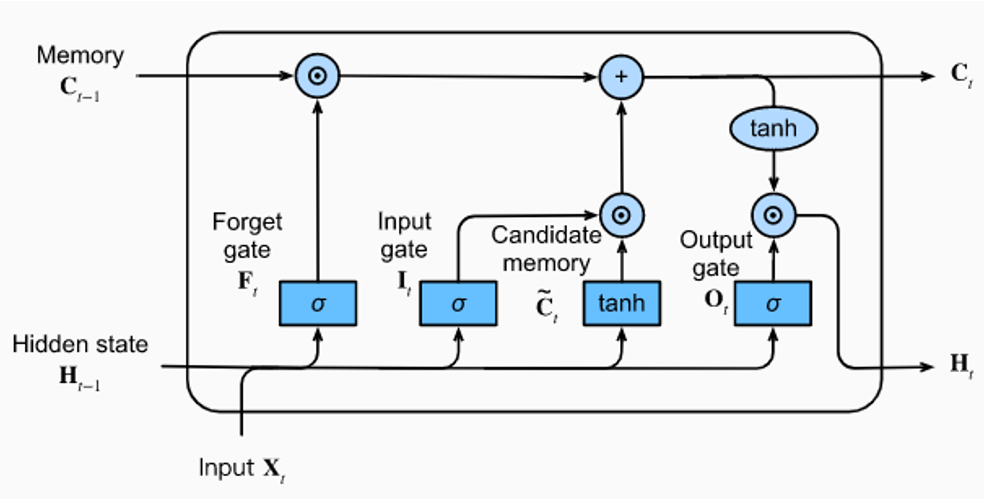
\includegraphics[width=0.8\textwidth]{figure/lstm.png}
        \caption{Structure of a Long Short-Term Memory (LSTM) Network}
        \label{figure:lstm_structure}
    \end{figure}
\end{frame}

\begin{frame}{ML Foundations: LSTM Performance}
    \begin{block}{LSTM's Information Flow}
        \begin{enumerate}
            \item \textbf{Forget Gate:} Determines retention or forgetting of previous cell state.
            \item \textbf{Input Gate:} Controls addition of new information to the cell state.
            \item \textbf{Memory Cell:} Stores and updates information based on input and previous state.
            \item \textbf{Output Gate:} Determines the next hidden state based on input and cell state.
        \end{enumerate}
    \end{block}

    \begin{block}{Performance}
        \begin{itemize}
            \item Demonstrated superior performance in capturing complex patterns and dependencies in sequential data.
            \item Valuable in various machine-learning applications, including time series forecasting.
        \end{itemize}
    \end{block}
\end{frame}

\begin{frame}{ML Foundations: RNN Overview}
    \begin{block}{Recurrent Neural Network (RNN)}\label{appx:rnn}
        \begin{itemize}
            \item Designed for sequential data processing, capturing dependencies across time.
            \item Connections form directed cycles, maintaining a hidden state for previous inputs.
            \item Faces vanishing gradient problem limiting long-term dependency capture.
        \end{itemize}
    \end{block}

    \begin{block}{Limitations}
        \begin{itemize}
            \item The Vanishing gradient problem hinders the ability to capture long-term dependencies.
            \item Overcome by more advanced architectures like Long Short-Term Memory (\hyperref[appx:lstm]{LSTM}) networks.
        \end{itemize}
    \end{block}
\end{frame}


\section{Results}

\begin{frame}{Exchange Rate Predictions: LSTM}
    \begin{columns}[T,onlytextwidth]
        \column{0.5\textwidth}
        \begin{figure}[ht]
            \centering
            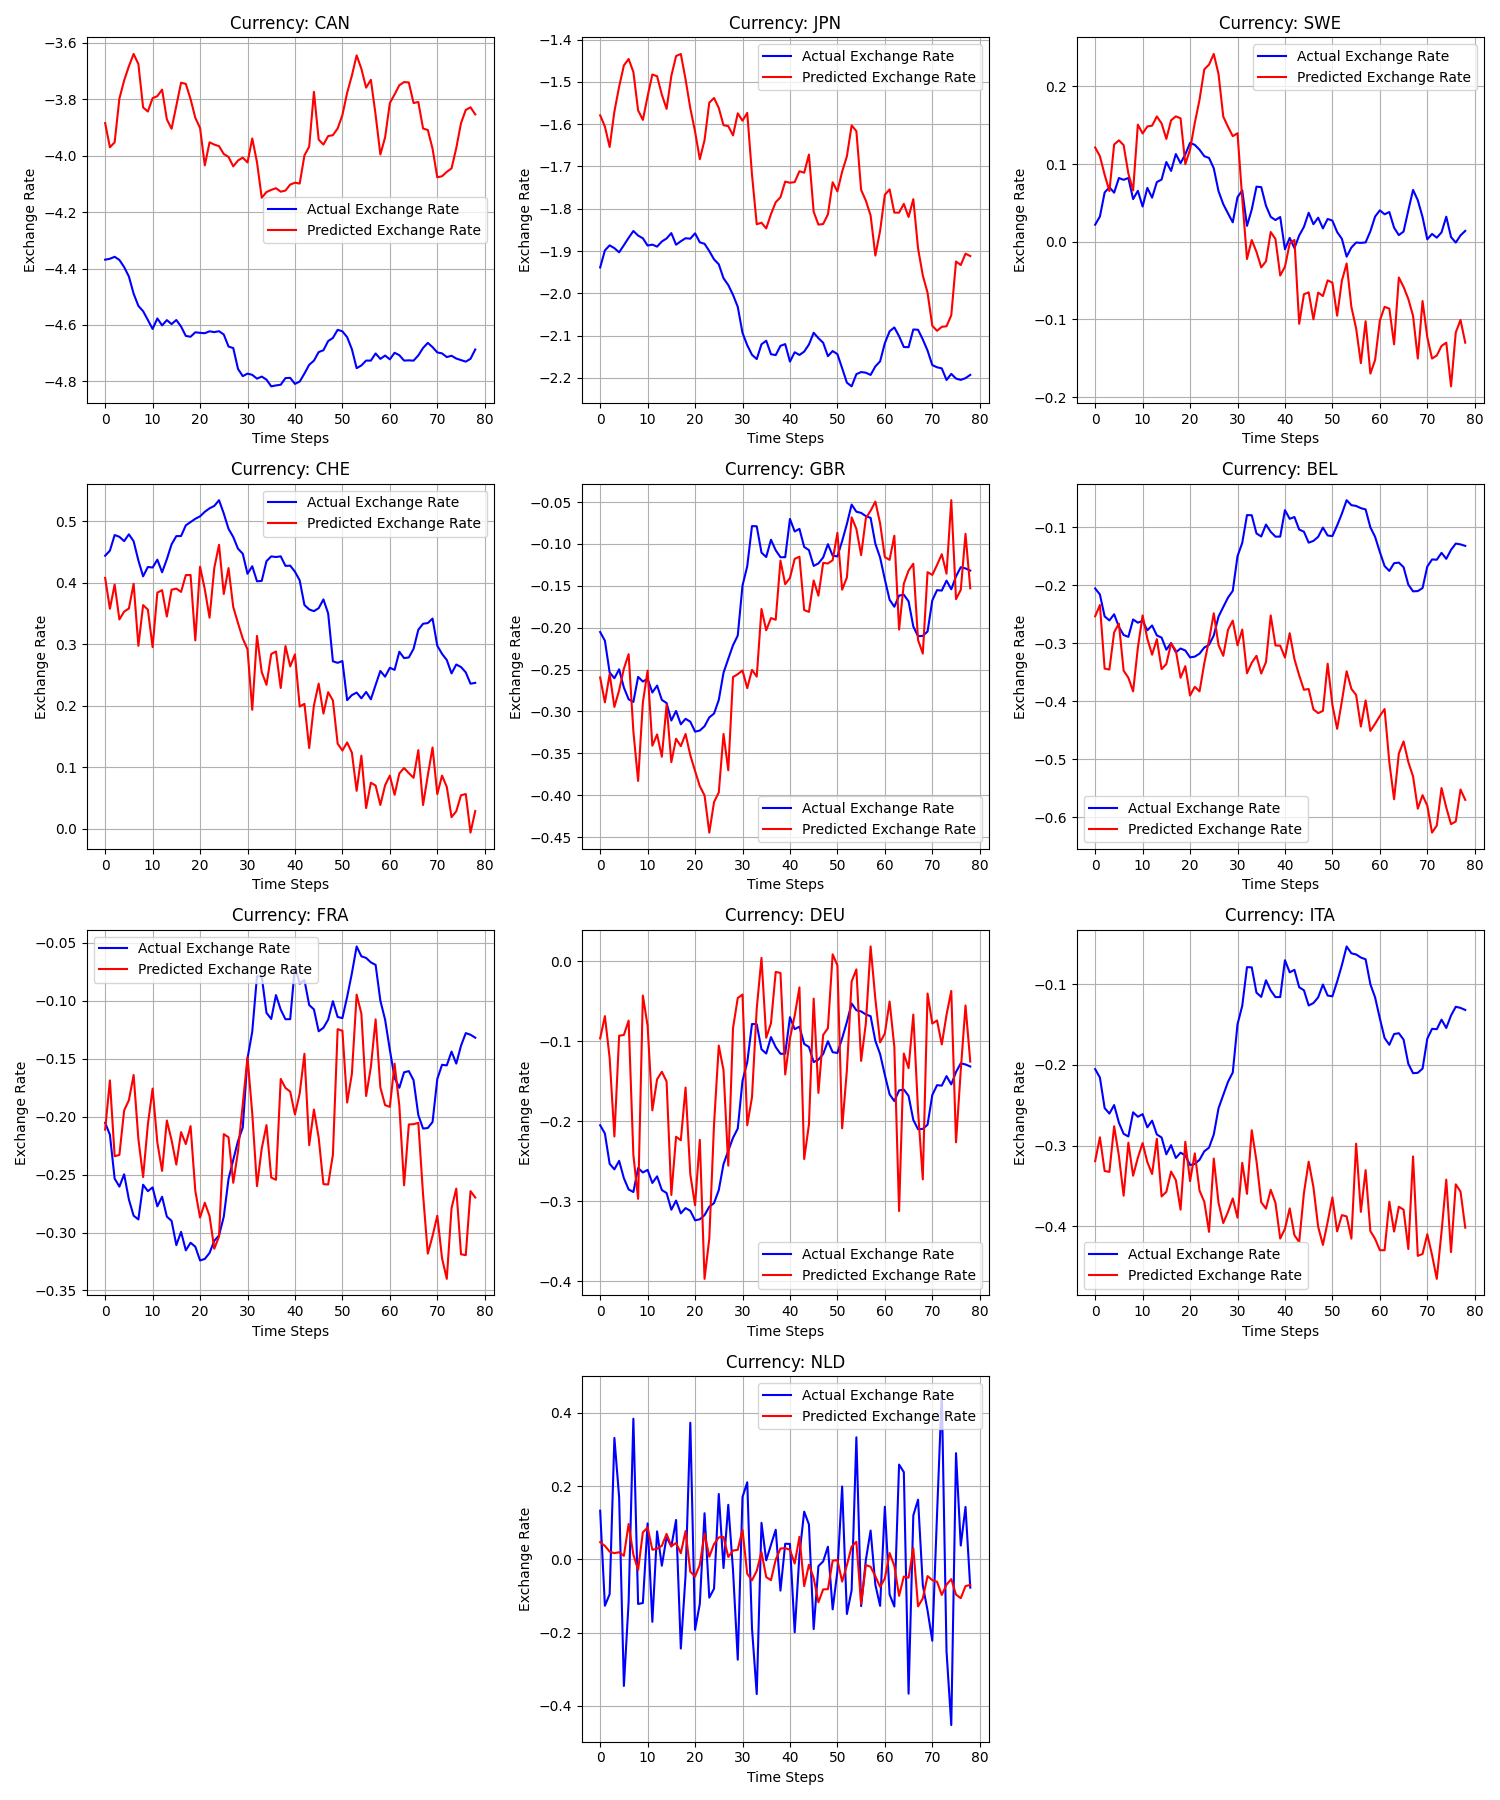
\includegraphics[width=\textwidth]{figure/lstm_exchange_rate_predictions.png}
            \caption{LSTM Exchange Rate Predictions}
            \label{figure:lstm_predictions}
        \end{figure}

        \column{0.45\textwidth}
        \begin{block}{Observations}
            LSTM model: Good at estimating levels and capturing long-term trends but struggles with sudden jumps.
        \end{block}
    \end{columns}
\end{frame}

\begin{frame}{Exchange Rate Predictions: RNN}
    \begin{columns}[T,onlytextwidth]
        \column{0.5\textwidth}
        \begin{figure}[ht]
            \centering
            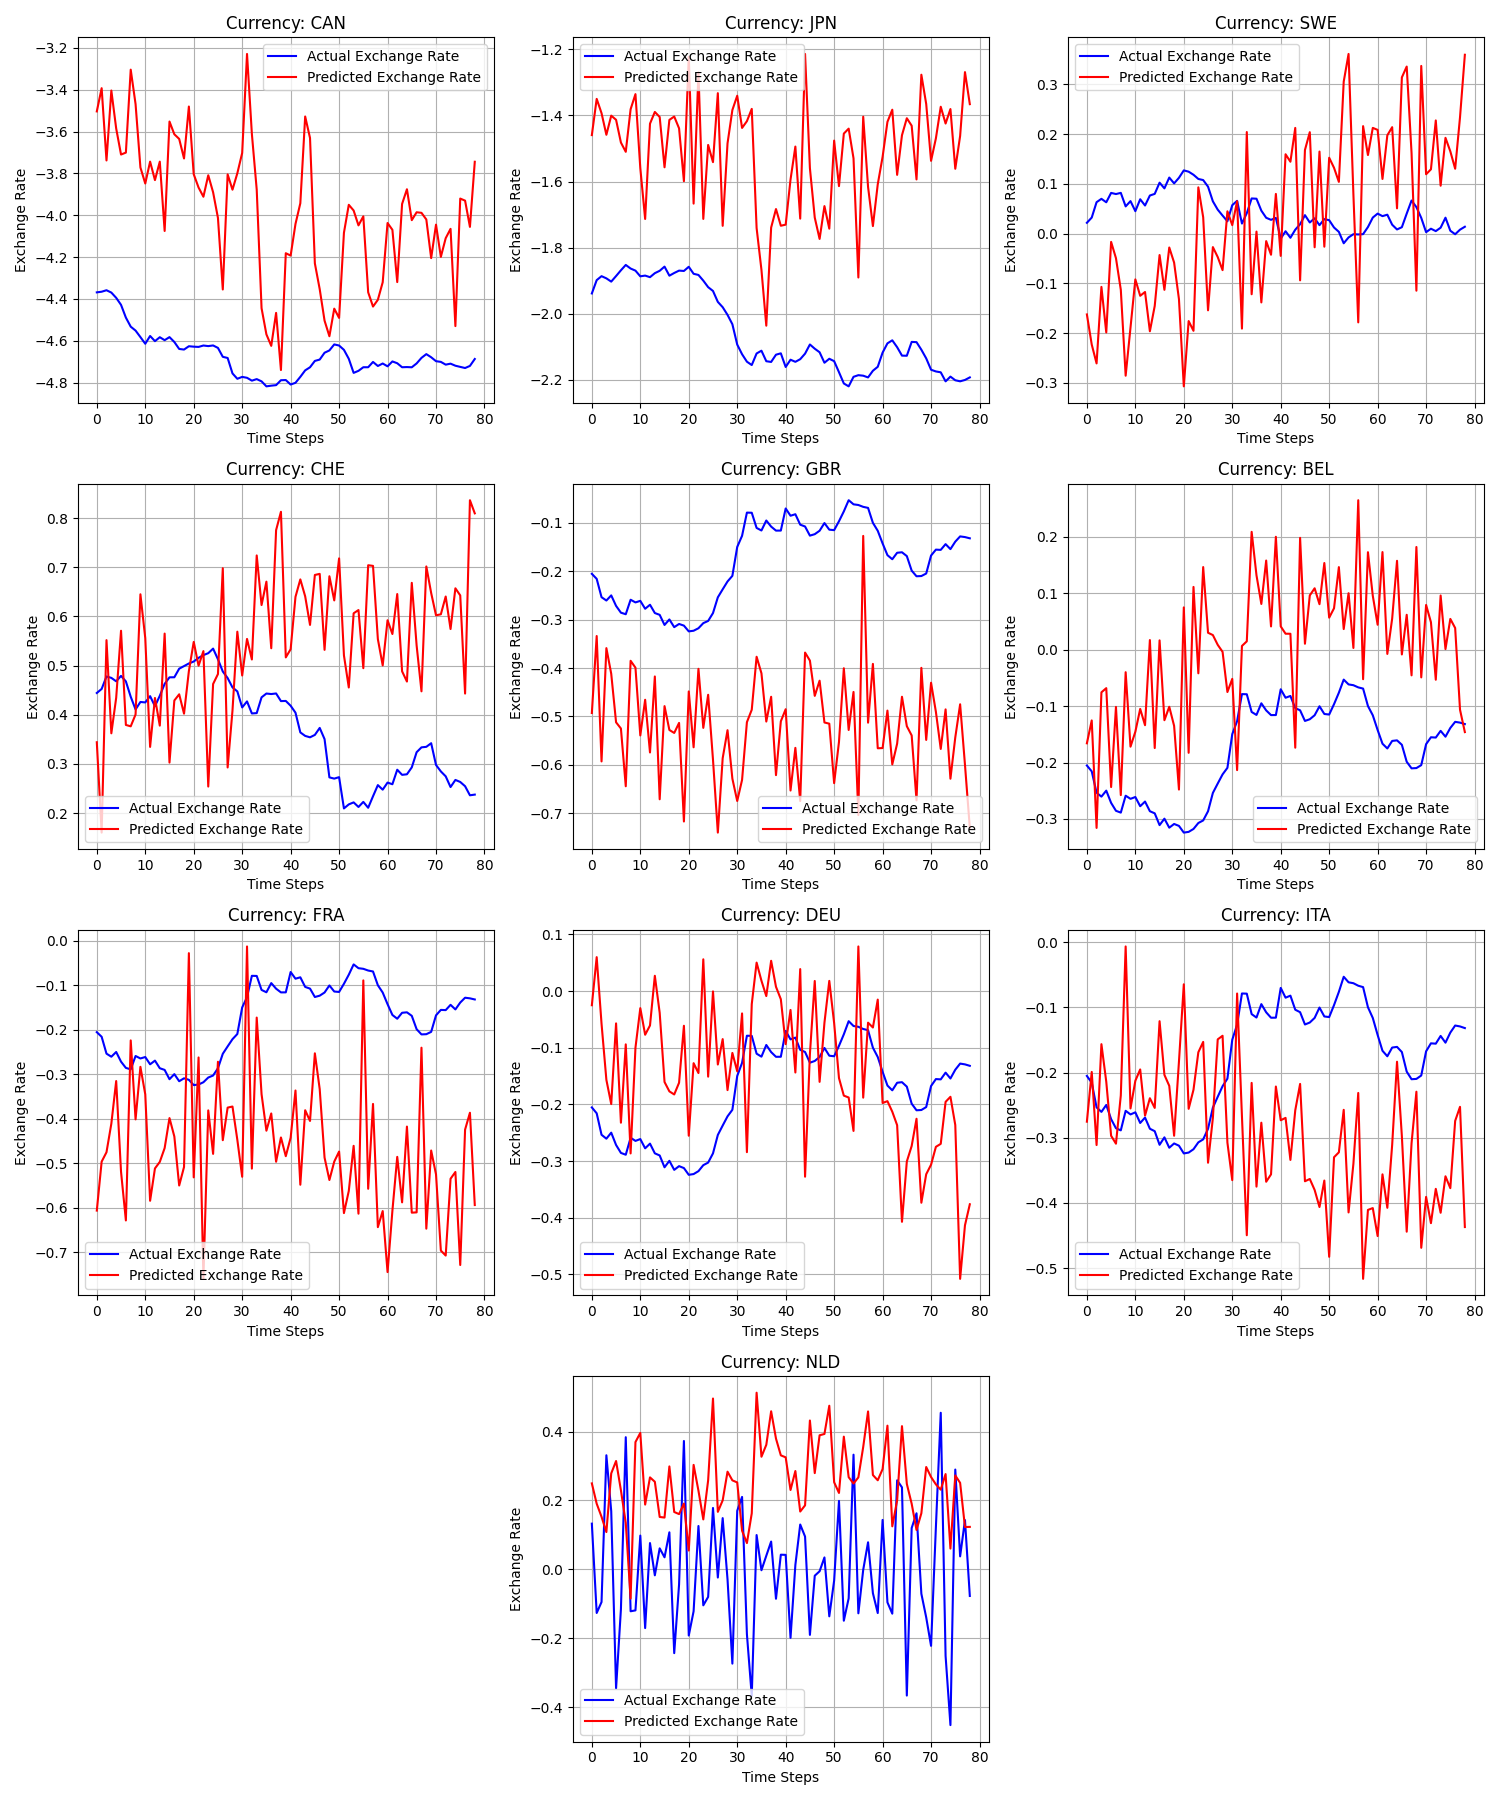
\includegraphics[width=\textwidth]{figure/rnn_exchange_rate_predictions.png}
            \caption{RNN Exchange Rate Predictions}
            \label{figure:rnn_predictions}
        \end{figure}

        \column{0.45\textwidth}
        \begin{block}{Observations}
            RNN model: Challenges in capturing both long-term trends and short-term fluctuations, especially in predicting jumps.
        \end{block}
    \end{columns}
\end{frame}

\begin{frame}{1/N Strategy Results}
    \begin{alertblock}{Comparison on 1/N Strategy}
        \begin{itemize}
            \item Absolute returns presented as percentages.
            \item Results for four different periods: 2012–2015, 2013–2016, 2014–2017, 2015–2018.
        \end{itemize}
    \end{alertblock}
\end{frame}

\begin{frame}{Results for 2012-2015}
    \begin{table}[h]
        \centering
        \csvautotabular{table/result_2012-07-31_2015-12-31.csv}
        \caption{Results for 2012–2015}
        \label{tab:results_2012-07-31_2015-12-31}
    \end{table}
\end{frame}

\begin{frame}{Results for 2013-2016}
    \begin{table}[h]
        \centering
        \csvautotabular{table/result_2013-01-31_2016-12-31.csv}
        \caption{Results for 2013–2016}
        \label{tab:results_2013-01-31_2016-12-31}
    \end{table}
\end{frame}

\begin{frame}{Results for 2014-2017}
    \begin{table}[h]
        \centering
        \csvautotabular{table/result_2014-01-31_2017-12-31.csv}
        \caption{Results for 2014–2017}
        \label{tab:results_2014-01-31_2017-12-31}
    \end{table}
\end{frame}

\begin{frame}{Results for 2015-2018}
    \begin{table}[h]
        \centering
        \csvautotabular{table/result_2015-01-31_2018-12-31.csv}
        \caption{Results for 2015–2018}
        \label{tab:results_2015-01-31_2018-12-31}
    \end{table}
\end{frame}

\section{Analysis of Results}

\begin{frame}{Model Performance Overview}
    \begin{block}{Key Findings}
        \begin{itemize}
            \item Consistently negative log returns, absolute returns, and alarming Sharpe ratios.
            \item Lack of positive returns indicated by the Gain/Loss Ratio.
            \item Possible reasons: inadequate model complexity, inappropriate parameter tuning, and absence of crucial features.
        \end{itemize}
    \end{block}

    \begin{block}{Limitations and Suggestions}
        \begin{itemize}
            \item Highly negative skewness and kurtosis values suggest difficulty capturing extreme market events.
            \item Additional features like monthly realised volatility may enhance model performance.
            \item Further investigation into incorporating relevant features for improved model dynamics.
        \end{itemize}
    \end{block}
\end{frame}

\begin{frame}{TVECM Dominance Exploration}
    \begin{block}{Observations}
        \begin{itemize}
            \item TVECM is the best-performing model among the considered ones.
            \item Speculative explanations for TVECM's dominance:
                \begin{itemize}
                    \item Long-term dynamics capture.
                    \item Adaptability to structural changes.
                    \item Strong cointegration patterns in data.
                    \item Parameter sensitivity and model simplicity.
                \end{itemize}
            \item Detailed analysis requires examining model specifications, data, and additional information.
        \end{itemize}
    \end{block}
\end{frame}

\begin{frame}{Comparison with Wang et al.}
    \begin{block}{LSTM vs. TVECM}
        \begin{itemize}
            \item Contrary to Wang et al.'s study, TVECM outperformed LSTM.
            \item Discrepancy may stem from differences in model specifications, data, or economic conditions.
        \end{itemize}
    \end{block}

    \begin{block}{Consistent Superiority}
        \begin{itemize}
            \item LSTM demonstrated consistent superiority over RNN and VAR.
            \item Aligns with broader trends observed in Wang et al.'s study.
        \end{itemize}
    \end{block}
\end{frame}

\begin{frame}{Performance Dynamics Over Time}
    \begin{block}{Key Trends}
        \begin{itemize}
            \item LSTM's performance relative to TVECM varied over different time periods.
            \item LSTM performed better as we moved further from the trained data.
            \item Implication: TVECM may degenerate faster than LSTM in severe market conditions.
        \end{itemize}
    \end{block}
\end{frame}

\begin{frame}{Realised Returns at Currency Pair Level}
    \begin{block}{Insights}
        \begin{itemize}
            \item Lack of specific information on realised volatility at the exchange rate level.
            \item Exploring this aspect could provide deeper insights into factors influencing LSTM's conflicting strategies.
        \end{itemize}
    \end{block}
\end{frame}

\section{Conclusion}

\begin{frame}{Conclusion}
    \begin{block}{Contributions}
        \begin{itemize}
            \item Introduction of LSTM networks for carry trade return prediction.
            \item LSTM's unique ability to capture long-term data patterns.
            \item Analysis spanning G10 currencies (1990-2019) shows LSTM underperformed traditional models.
        \end{itemize}
    \end{block}

    \begin{block}{Key Findings}
        \begin{itemize}
            \item Deterioration in carry trade returns post-2008 crisis supports the UIP hypothesis.
            \item LSTM underperformance during 2015-2018 prompts deeper investigation.
        \end{itemize}
    \end{block}
\end{frame}

\begin{frame}{Implications}
    \begin{block}{Implications and Future Research}
        \begin{itemize}
            \item Explore long-term trends, structural changes, and evolving market dynamics.
            \item Macro-economic analysis and applicability of LSTM in various economic settings.
            \item Nuanced features of carry trade returns in post-financial crisis conditions.
        \end{itemize}
    \end{block}
\end{frame}

%---------------------------------------------------------

% Specify the bibliography style and file
\bibliographystyle{unsrt}
\bibliography{references}

\end{document}
